% !TEX option = -shell-escape
% Important: The shell-escape flag is required for the Minted package.
% Please compile this document with 'pdflatex -shell-escape main.tex'.
% If you are using another IDE, you may be able to specify this in the
% options or to provide an option like '% !TEX option = -shell-escape'
% in this file, depending on your builder. See the README.md for more.

% Don't put any content in here.
% Don't even include content files by using \input or \inlcude.
% Put your content into components/text.tex or include it there using \input.
% You probably want to modify the following files:
%   components/info.tex             contains the author, title etc.
%   components/settings.tex         contains the packages and settings.
%   components/commands.tex         contains helpful custom commands.
%   components/glossary.tex         contains an explanation of the used terms.
%   components/acknowledgements.tex contains the acknowledgements.
%   components/quote.tex            contains a quote.
%   components/abstract.tex         contains the abstract of the document.
%   components/text.tex             includes the actual content of the document.
%   components/outline.tex          contains the outline.
%   components/preface.tex          contains the preface.
%   chapters/                       contains the main text.
%   bibliography/literature.bib     contains the BibTeX entries.
%   images/                         contains all your content-related images.
%
% You probably don't need to change anything in the following files:
%   components/cover.tex            formats the front cover of the document.
%   components/titlepage.tex        formats the title page of the document.
%   components/disclaimer.tex       formats the disclaimer page.
%   styles/                         contains style elements (e.g. logos).
%   main.tex                        contains the top-level code structure.
%   README.md                       contains information about this template.

\documentclass[11pt,
              a4paper,
              index=totoc,
              headsepline,
              footsepline,
              BCOR=12mm,
              DIV=13]{scrbook}

% KOMA scrbook options:
%  index=totoc: include an entry for the index in the table of contents.
%  headsepline: use horizontal line under heading.
%  footsepline: use horizontal line above footer.
%  BCOR: binding correction (e.g.: BCOR=12mm)
%  DIV: Number of sheet sections (used for layout) (e.g.: DIV=13)


%  This code base is currently hosted at: 
%  https://github.com/waltsims/TUM_Thesis_Template_CSE
             
% !TEX root = ../main.tex
% Set here the title, authors and other stuff to be used for the cover
% This file is used by MAIN.TEX

% set title, authors and stuff for the cover
\def\university{Technische Universit{\"a}t M{\"u}nchen}
\def\universityLogo{styles/tum_logo}
\def\program{Computational Science and Engineering \\(International Master's Program)}
\def\programLogo{styles/cse_logo}
\def\doctype{Master's Thesis}

\def\title{Temporary}
\def\author{Stephen Ryan}
\def\examinerOne{Univ.-Prof.\ Dr.\ Qui-Gon Jinn}
\def\examinerTwo{Univ.-Prof.\ Dr.\ Obi-Wan Kenobi}
\def\assistantAdvisor{Dr.\ rer.\ nat.\ Anakin Skywalker}
\def\date{May 4th, 2420}

\def\keywords{{keyword1}, {keyword2}, {keyword3}}

% The following are used for the PDF metadata, by default the same as above.
\def\metaTitle{\title}
\def\metaAuthor{\author}
\def\metaSubject{\doctype\ -\ \university}
\def\metaKeywords{\keywords}

% text to appear in the footer
\def\footertext{}


% !TEX root = ../main.tex
% Included by MAIN.TEX

%--------------------------------------------------
% Fonts and page setup
%--------------------------------------------------

% Default font
\usepackage{palatino}

\usepackage[utf8]{inputenc}

% Enable special PostScript fonts (optional)
% \usepackage{pifont}

% Manipulate the footer
\usepackage{scrlayer-scrpage}
\usepackage{scrhack}
\pagestyle{scrheadings}
\ifoot[\footertext]{\footertext} % \footertext set in INFO.TEX

% Set the font for the section headings
\renewcommand{\sectfont}{\normalfont \bfseries}

% Conditional commands in LaTeX documents, used for the \clearemptydoublepage.
\usepackage{ifthen}

% Typeset text in multiple columns (optional)
% \usepackage{multicol}

% Rotation tools, including rotated full-page floats (optional)
\usepackage{rotating}


%--------------------------------------------------
% Document structure
%--------------------------------------------------

% Pro­duce hy­per­text links in the doc­u­ment (recommended)
\usepackage{hyperref}

% Create glossaries and lists of acronyms
% depending on how many packages were shipped with your TeX distribution,
% you might need to install xindy. On Linux: sudo apt install xindy
\usepackage[toc, xindy]{glossaries}

% Standard LaTeX package for creating indexes
\usepackage{makeidx}


%--------------------------------------------------
% Bibliography
%--------------------------------------------------

% Set the bibliography style (default: plain)
\bibliographystyle{plain}

% Special biblography package (nice to have)
% \usepackage{natbib}


%--------------------------------------------------
% Graphics and floats
%--------------------------------------------------

% Enhanced support for graphics (recommended)
\usepackage{graphicx}
% Path to the figures directory (default: {figures/})
% Multiple entries are allowed, e.g. {{figures1/}{figures2/}}.
\graphicspath{{figures/}}

% Improved interface for floating objects (optional)
\usepackage{float}

% To use the subfigures (optional)
\usepackage{subcaption}


%--------------------------------------------------
% Mathematics
%--------------------------------------------------

% AMS mathematical facilities for LaTeX (recommended)
\usepackage{amsmath}

% TeX fonts from the American Mathematical Society (recommended)
\usepackage{amsfonts}

% Some extra math symbols (optional)
% \usepackage{amssymb}

% Extended maths fonts for LaTeX (optional)
% \usepackage{yhmath}

% Provide math delimiters whose size can be computed automatically (optional)
% \usepackage{commath}


%--------------------------------------------------
% Source code and algorithms
%--------------------------------------------------

% Source code typesetting
% \usepackage{listings} % (optional - alternative)
\usepackage[newfloat]{minted} % (recommended)
% Set global Minted options
\setminted{linenos, autogobble, frame=lines, framesep=2mm}
% Inline C++ (optional)
\newcommand{\incpp}[1]{\mintinline{c++}{#1}}
\newenvironment{code}{\captionsetup{type=listing}}{}
\SetupFloatingEnvironment{listing}{name=Source Code}

% Typeset algorithms - pseudocode (optional)
\usepackage{algorithm}
\usepackage{algpseudocode}
% Normal arrow comments
% \algrenewcommand{\algorithmiccomment}[1]{\hfill$\rightarrow$ #1}


%--------------------------------------------------
% Tables
%--------------------------------------------------

% Tables (optional)
\usepackage{tabu}

% Add color to LaTeX tables (optional)
% \usepackage{colortbl}

% Create tabular cells spanning multiple rows (optional)
% \usepackage{multirow}


%--------------------------------------------------
% Color
%--------------------------------------------------

% Use colors
\usepackage[dvipsnames]{xcolor}

% You may find all the pre-defined colors in
% https://en.wikibooks.org/wiki/LaTeX/Colors#Predefined_colors

% Custom colors
\definecolor{Pantone300C}{HTML}{0065BD} % TUM primary blue
\definecolor{Pantone301}{HTML}{005293}  % TUM secondary light blue
\definecolor{Pantone540}{HTML}{003359}  % TUM secondary dark blue
\definecolor{DarkGray}{HTML}{333333}    % TUM secondary dark gray
\definecolor{MediumGray}{HTML}{808080}  % TUM secondary medium gray
\definecolor{LightGray}{HTML}{CCCCC6}   % TUM secondary light gray
\definecolor{Pantone7527}{HTML}{DAD7CB} % TUM accent gray
\definecolor{Pantone158}{HTML}{E37222}  % TUM accent orange
\definecolor{Pantone383}{HTML}{A2AD00}  % TUM accent green
\definecolor{Pantone283}{HTML}{98C6EA}  % TUM accent very light blue
\definecolor{Pantone542}{HTML}{64A0C8}  % TUM accent light blue

% Color for the hyperlinks (e.g. table of contents)
\def\colorLinks{Pantone300C}
% Color for the web links
\def\colorUrl{Pantone542}
% Color for the citations
\def\colorCitations{Pantone158}

%--------------------------------------------------
% PDF output
%--------------------------------------------------

% Adjust the color of the links
\hypersetup{
  linkcolor=\colorLinks,%
  urlcolor=\colorUrl,%
  citecolor=\colorCitations
}

% Disable the coloring of the links when printing.
% Requires a compatible PDF reader.
\usepackage[ocgcolorlinks]{ocgx2}[2017/03/30]

% PDF Metadata
\hypersetup{
  pdftitle={\metaTitle},%
  pdfauthor={\metaAuthor},%
  pdfkeywords={\metaKeywords},%
  pdfsubject={\metaSubject}
}

% Create XMP Metadata (uses the values from hyperref)
\usepackage{hyperxmp}

% Make thumbnails (optional)
% \usepackage{thumbpdf}


%--------------------------------------------------
% Other settings
%--------------------------------------------------

% Define commands that appear not to eat spaces (optional)
\usepackage{xspace}

\usepackage{tikz}
\usepackage{circuitikz}
\usetikzlibrary{patterns}
\tikzstyle{load}   = [ultra thick,-latex]
\tikzstyle{stress} = [-latex]
\tikzstyle{dim}    = [latex-latex]
\tikzstyle{axis}   = [-latex,black!55]

% !TEX root = ../main.tex
% Included by MAIN.TEX
% Please include your own cool commands here.
% Be only sure to comment it sufficiently so others can use it.

%-------------------------------------------------------------
%                      Own Commands
%-------------------------------------------------------------


%-------------------------------------------------------------
% math stuff -------------------------------------------------

% nice R, N, C
\newcommand{\nat}{\mathbb{N}}
\newcommand{\real}{\mathbb{R}}
\newcommand{\compl}{\mathbb{C}}

% un demi
\newcommand{\half}{\frac{1}{2}}

% parantheses
\newcommand{\parenth}[1]{ \left(#1 \right) }
\newcommand{\bracket}[1]{ \left[#1 \right] }
\newcommand{\accolade}[1]{ \left\{ #1 \right\} }
%\newcommand{\angle}[1]{ \left\langle  #1 \right\rangle }

% partial derivative: %#1 function, #2 which variable
% simple / single line version
\newcommand{\pardevS}[2]{ \delta_{#1} f(#2) }

% fraction version
\newcommand{\pardevF}[2]{ \frac{\partial #1}{\partial #2} }

% render vectors: 3 and 4 dimensional
\newcommand{\veciii}[3]{\left[ \begin{array}[h]{c} #1 \\ #2 \\ #3	\end{array} \right]}
\newcommand{\veciv}[4]{\left[ \begin{array}[h]{c} #1 \\ #2 \\ #3 \\ #4	\end{array} \right]}

% render matrices: 3  dimensional (arguments in row first order)
\newcommand{\matiii}[9]{\left[ \begin{array}[h]{ccc} #1 & #2 & #3 \\ #4 & #5 & #6 \\ #7 & #8 & #9	\end{array} \right]}

%-------------------------------------------------------------
% some abreviations ------------------------------------------
\newcommand{\Reg}{$^{\textregistered}$}
\newcommand{\reg}{$^{\textregistered}$ }
\newcommand{\Tm}{\texttrademark}
\newcommand{\tm}{\texttrademark~}
\newcommand {\bsl} {$\backslash$}

%-------------------------------------------------------------
% formating --------------------------------------------------

% Theorem & Co environments and counters
\newtheorem{theorem}{Theorem}[chapter]
\newtheorem{lemma}[theorem]{Lemma}
\newtheorem{corollary}[theorem]{Corollary}
\newtheorem{remark}[theorem]{Remark}
\newtheorem{definition}[theorem]{Definition}
\newtheorem{equat}[theorem]{Equation}
\newtheorem{example}[theorem]{Example}
%\newtheorem{algorithm}[theorem]{Algorithm}

% inserting figures
\newcommand{\insertfigure}[4]{ % Filename, Caption, Label, Width percent of textwidth
	\begin{figure}[htbp]
		\begin{center}
			\includegraphics[width=#4\textwidth]{#1}
		\end{center}
		\vspace{-0.4cm}
		\caption{#2}
		\label{#3}
	\end{figure}
}

% referecing figures

\newcommand{\refFigure}[1]{ %label
	Figure~\ref{#1}
}
\newcommand{\refChapter}[1]{ %label
	Chapter~\ref{#1}
}

\newcommand{\refSection}[1]{ %label
	Section~\ref{#1}
}

\newcommand{\refParagraph}[1]{ %label
	Paragraph~\ref{#1}
}

\newcommand{\refEquation}[1]{ %label
	Equation~\ref{#1}
}

\newcommand{\refTable}[1]{ %label
	Table~\ref{#1}
}

\newcommand{\rigidTransform}[2]
{
	${}^{#2}\!\mathbf{H}_{#1}$
}

% comment that appears on the border - very practical !!!
\newcommand{\comment}[1]{\marginpar{\raggedright \noindent \footnotesize {\textsl{#1}} }}

% page clearing
\newcommand{\clearemptydoublepage}{%
  \ifthenelse{\boolean{@twoside}}{\newpage{\pagestyle{empty}\cleardoublepage}}%
  {\clearpage}}

%-------------------------------------------------------------
%-------------------------------------------------------------

\newcommand{\etAl}{\emph{et al.}\mbox{ }}


% !TEX root = ../main.tex
\newglossaryentry{computer}
{
  name=computer,
  description={is a programmable machine that receives input,
               stores and manipulates data, and provides
               output in a useful format}
}

\newglossaryentry{poc}
{
  name={proof of concept},
  description={}
  }
\newglossaryentry{ui}
{
  name={user interface},
  description={}
  }
\newglossaryentry{ai}
{
  name={arithmetic intensity},
  description={a measure of floating-point operations (FLOPs)
              \hyphenation{per-formed} performed by a \hyphenation{gi-ven} given code or code section relative
              to the amount of memory accesses (Bytes) that are required
               to support those operations\cite{AI}}
  }

\newglossaryentry{speed-up}
{
  name={speed-up},
  description={the factor of temporal acceleration a program
  exhibits when additional computational resources are dedicated to it's execution.}
}

\newglossaryentry{directive pragmas}
{
  name={directive pragma},
  description={a computer programming language construct that specifies how a compiler
  should process input data} % sourced from wikipedia
}


\newglossaryentry{rc}{%SOURCE: wikipedia
name={race condition},
description={A race condition or race hazard is the behavior of an electronic,
 software, or other system where the output is dependent on the sequence or
 timing of other uncontrollable events. It becomes a bug when events do not
 happen in the order the programmer intended. The term originates with the idea
 of two signals racing each other to influence the output first.}
}
\newglossaryentry{dd}{
name={data dependencies},
description={}
}
\newglossaryentry{sisd}{
name={single instruction single data},
description={}
}
\newglossaryentry{simt}{
name={single instruction multiple threads},
description={}
}

\newglossaryentry{simd}{
name={single instruction multiple data},
description={}
}
\newglossaryentry{gp}{%SOURCE: wikipedia
name={Gaussian Plane},
description={The two dimensional plane of complex numbers.}
}
\newglossaryentry{CURAND}{
name={CURAND},
description={
The CURAND library provides facilities that focus on the simple and efficient
generation of high-quality pseudorandom and quasirandom numbers.\cite{cuRAND}
}
}

\newacronym[longplural={partial differential equations}]{PDE}{PDE}{partial differential equations}
\newacronym{mpi}{MPI}{Message Passing Interface}

\newacronym[longplural={Random Walks on Spheres}]{RWoS}{RWoS}{Random Walk on Spheres}

\newacronym[longplural={graphical processing units}]{GPU}{GPU}{graphical processing unit}

\newacronym[longplural={central processing units}]{CPU}{CPU}{central processing unit}
\newacronym{hpc}{HPC}{high performance computing}

\newacronym[longplural={arithmetic logic units}]{ALU}{ALU}{arithmetic logic unit}

\newacronym[longplural={streaming multi-processors}]{SM}{SM}{streaming multi-processor}

\newacronym[longplural={boundary value problems}]{BVP}{BVP}{boundary value problem}
\newacronym[longplural={general purpose graphical processing units}]{GPGPU}{GPGPU}{general purpose graphical processing units}
\newacronym{CUDA}{CUDA}{compute unified device architecture}
\newacronym{RAM}{RAM}{random access memory}
\newacronym{SRAM}{SRAM}{static random access memory}
\newacronym{DRAM}{DRAM}{dynamic random access memory}
\newacronym{I/O}{I/O}{input/output}
\newacronym{PTX}{PTX}{Parallel Thread eXecution}
\newacronym{jit}{JIT}{just in time}


\makeglossaries

\begin{document}

 \frontmatter

 % !TEX root = ../main.tex
% The front cover.
% Included by MAIN.TEX

%--------------------------------------------------
% The Front Cover
%--------------------------------------------------

% correct BCOR - undo at the end !!!
\def\bcorcor{0.15cm}
\addtolength{\hoffset}{\bcorcor}

\thispagestyle{empty}

\vspace{4cm}
\begin{center}
	\includegraphics[width=4cm]{\universityLogo}\\
	\vspace{5mm}
	\huge \program \\
	\vspace{0.5cm}
	\large \university
\end{center}

\vspace{20mm}
\begin{center}
	{\Large \doctype}\\
	\vspace{20mm}
	{\huge \textbf \title}\\
	\vspace{15mm}
	{\LARGE  \author}\\
	\vspace{\fill}
	% \includegraphics[width=4cm]{\programLogo}
\end{center}


 \clearemptydoublepage

 % !TEX root = ../main.tex
% The titlepage.
% Included by MAIN.TEX


%--------------------------------------------------
% The title page
%--------------------------------------------------

% correct BCOR - undo at the end !!!
\def\bcorcor{0.15cm}
\addtolength{\hoffset}{\bcorcor}

\thispagestyle{empty}

\vspace{4cm}
\begin{center}
    \includegraphics[width=4cm]{\universityLogo}\\
    \vspace{5mm}
    \huge \program \\
    \vspace{0.5cm}
    \large \university
\end{center}

\vspace{10mm}
\begin{center}
    {\Large \doctype}\\
    \vspace{10mm}
    {\LARGE \title}\\
    \vspace{10mm}

    \begin{tabular}{ll}
      \Large Author:                        & \Large \author \\[2mm]
      \Large 1\textsuperscript{st} examiner:& \Large \examinerOne\\[2mm]
      \Large 2\textsuperscript{nd} examiner:& \Large \examinerTwo \\[2mm]
      \Large Assistant advisor:             & \Large \assistantAdvisor \\[2mm]
      \Large Submission Date:               & \Large \date
    \end{tabular}

    \vspace{\fill}
    \includegraphics[width=4cm]{\programLogo}
\end{center}

% undo BCOR correction
\addtolength{\hoffset}{\bcorcor}


 % !TEX root = ../main.tex
\clearemptydoublepage

\thispagestyle{empty}
\vspace*{0.8\textheight}
\noindent
I hereby declare that this thesis is entirely the result of my own work except where otherwise indicated. I have only used the resources given in the list of references.

\vspace{15mm}
\noindent
\date \hspace{5cm} \author
\newpage


 % !TEX root = ../main.tex
\clearemptydoublepage
\phantomsection
\addcontentsline{toc}{chapter}{Acknowledgements}

\vspace*{2cm}

\begin{center}
{\Large \textbf{Acknowledgments}}
\end{center}

\vspace{1cm}

\begin{center}
If someone helped you or supported you through your studies, this page is a
good place to tell them how thankful you are.
\end{center}


 \clearpage
\phantomsection

\begin{center}
\vspace*{11cm}
\textit{``People sometimes ask me if it is a sin in the Church of Emacs to use vi.
	Using a free version of vi is not a sin; it is a penance. So happy hacking''}
\end{center}
\par
\hspace*{7cm}
\textit{-Richard Stallman}


 % !TEX root = ../main.tex
% The abstract.
% Included by MAIN.TEX
\clearemptydoublepage
\phantomsection
\addcontentsline{toc}{chapter}{Abstract}

\vspace*{2cm}
\begin{center}
{\Large \textbf{Abstract}}
\end{center}
\vspace{1cm}

This document will serve as an example to you, of how to use \LaTeX to write your
CSE Master's Thesis. It will have examples and recomendations, and hopefully a
few laughs.  Because this is the abstract, it will have to convince you that this 
template is something you want to use.  It has been proven, that without using
this template, writing your thesis will be much more dificult. The template is
based on previous work, and has been improved apon and updated.  The result of 
this template is a modern latex template that everyone can contribute to and use
for their studies of CSE @ TUM.

Some more great abstract tips can be found here: 
\href{https://users.ece.cmu.edu/~koopman/essays/abstract.html}{Great Abstract tips}


 \tableofcontents

 \mainmatter

 % !TEX root = ../main.tex
% Included by MAIN.TEX
% Put your content in here or include it by using \input (\include won't work)

\addtolength{\evensidemargin}{-12mm}

% ---------------------------------------------------------------------------
%
%Introduction and Background Theory
%
% ---------------------------------------------------------------------------
\part[Introduction and Background Theory]{Introduction and Background Theory}
\label{part:introAndBackgroundTheory}
% !TEX root = ../main.tex
\chapter{Introduction}
\label{chapter:Introduction}
% This document has been created in order to show you some of the capabilities 
% of \LaTeX.  A great resource for an introduction to \LaTeX\xspace is Tobias
% Oetiker's ''The Not So Short Introduction to \LaTeXe'' \cite{latex}.  Please
% page through that document
% before starting with your thesis.
% Oh, and let's use the mysterious word \gls{computer} here to give the glossary
% a reason to appear.
% A third useful option to reference stuff besides citing or glossarying (?) 
% is using footnotes. Just like
% this\footnote{Properly formatted clickable URL: \url{https://www.tum.de/}}
% one.
% And: lists! Lists with bullet points are amazing. I mean, just look at this:
% \begin{itemize}
% 	\item list
% 	\item all 
% 	\item the 
% 	\item things!
% \end{itemize}
% % use enumerate for numbers instead of points: 
% % https://en.wikibooks.org/wiki/LaTeX/List_Structures#List_structures
% \par
% Anyways your introduction goes here.


% Below a few \LaTeX examples are included for beginners
% \comment{You can also put comments in the margins for you or your advisor}
% \begin{figure}[ht]
%   \centering
%   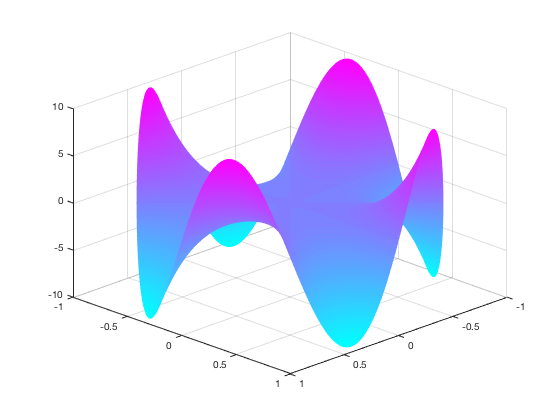
\includegraphics[width=5cm]{images/swing_function_plot.png}
%   \caption{$u(x)$}%{Numerically solved solution}
%   \label{fig:swingPlot}
% \end{figure}


% Equations can also be labeled
% \begin{equation}
% 	\pi = \mathrm{e}^{i\cdot\phi}
% 	\label{eq:equation1}
% \end{equation}


% And later referenced. Even in subfigures.
% \begin{figure}[!htb]
%   \centering
%   \begin{subfigure}[b]{0.3\textwidth}
%     \centering
%   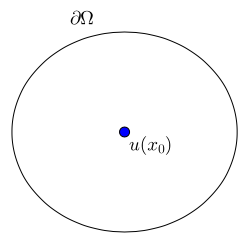
\includegraphics[width=\textwidth]{images/CircCenter}
%   \caption{Equation~\ref{eq:equation1}}\label{fig:circcenter}
% \end{subfigure}
% \hfill
%   \begin{subfigure}[b]{0.3\textwidth}
%     \centering
%   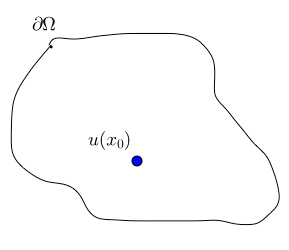
\includegraphics[width=\textwidth]{images/GeneralOffset}
%   \label{fig:generaloffset}
%   \caption{Equation~\ref{eq:equation1}}
% \end{subfigure}
% \end{figure}
% \section{Including code}

% Code can be using the package
% \href{https://www.sharelatex.com/learn/Code\_Highlighting\_with\_minted}{Minted}.

% An exaple of which of can be found below (see Source Code~\ref{lst:nice_listing})
% \begin{listing}
% 	%the language syntax can be declared here.
% 	\begin{minted}{python} 
% 	import numpy as np
	
% 	def incmatrix(genl1,genl2):
% 	    m = len(genl1)
% 	    n = len(genl2)
% 	    M = None #to become the incidence matrix
% 	    VT = np.zeros((n*m,1), int)  #dummy variable
	
% 	    #compute the bitwise xor matrix
% 	    M1 = bitxormatrix(genl1)
% 	    M2 = np.triu(bitxormatrix(genl2),1)
	
% 	    for i in range(m-1):
% 	        for j in range(i+1, m):
% 	            [r,c] = np.where(M2 == M1[i,j])
% 	            for k in range(len(r)):
% 	                VT[(i)*n + r[k]] = 1;
% 	                VT[(i)*n + c[k]] = 1;
% 	                VT[(j)*n + r[k]] = 1;
% 	                VT[(j)*n + c[k]] = 1;
	
% 	                if M is None:
% 	                    M = np.copy(VT)
% 	                else:
% 	                    M = np.concatenate((M, VT), 1)
	
% 	                VT = np.zeros((n*m,1), int)
	
% 	    return M
% 	\end{minted}

%   \caption{My nice listing}
%   \label{lst:nice_listing}
% \end{listing}

% !TEX root = ../main.tex

\chapter{Multigrid Methods}
\label{chapter:MultigridMethods}

\section{Smoothers}

% TODO: source Saad 2003

% TODO: define the linear problem Ax = b

% Quick comparison to direct
% TODO: fix the LU- QR- dash formatting if necessary. ALSO THIS SHOULD BE BEFORE THE SECTION ABOUT GMRES. (or maybe introduce multigrid first, then as preconditioner later?)
For the solution of sparse linear systems, two distinct types of methods, iterative and direct methods, can be applied. For general purposes, direct methods usually utilize various decomposition or factorization techniques such as LU, QR, or Cholesky in order to achieve a solution to machine precision in a known finite amount of steps. The number of steps necessary for methods such as LU decomposition is $O(n^3)$, which is increasingly disadvantageous for ever larger linear systems that are arising form the applicaiton of finite element methods.

% Advantages of relaxations: easy to implement, more general linear systems mgtut[23,24,26]
% (cf. Axelsson [6], Hackbusch [86], Varga [200])
Several variants of iterative methods exist, but for introducing and demonstrating the advantages multigrid methods, the focus will be on relaxation methods, such as Jacobi or Gauss-Seidel. These methods involve decomposition of the operator $A = D - L - U$ where $D$ is the diagonal of $A$, $-L$ is the strictly lower triangular part, and $-U$ is the strictly upper triangular part. The goal is then to use this decomposition to improve the starting guess $\mathbf{x}_{0}$, of the vector of unknowns $\mathbf{x}$ iteratively.

In the Jacobi scheme, rearranging after the decomposition of $A$ gives the iteration scheme

\begin{equation}
	\begin{aligned}
	\mathbf{x}^{(k+1)} &= D^{-1}(L + U)\mathbf{x}^{(k)} + D^{-1}\mathbf{b} \\ 
	                   &= R_J\mathbf{x}^{(k)} + D^{-1} \mathbf{b}
	\end{aligned}
\end{equation}

where matrix $R_J = D^{-1}(L + U)$ is defined as the Jacobi iteration matrix.

Component-wise, the updated $i$-th vector component can be obtained from the previous iteration's approximation of all other unknowns as:

\begin{equation}
	x_{i}^{(k+1)} = \frac{1}{a_{ii}}\left(b_i- \sum_{j \neq i}{a_{ij}x_{j}^{(k)}} \right).
\end{equation}

If the Jacobi method is initally used to compute an itermediate approximation, this can be weighted with a factor $\omega$ against the previous approximation, given in matrix form as

\begin{equation}
	\begin{aligned}
	\mathbf{x}^{(k+1)} &= \left[ (1-\omega) I + \omega R_J \right] \mathbf{x}^{(k)} + \omega D^{-1}\mathbf{b} \\
	&= R_{\omega}\mathbf{x}^{(k)} + \omega D^{-1} \mathbf{b}.
	\end{aligned}
\end{equation}

Different values of $\omega$ determines a factor known as the relaxtion rate which will be important to the idea of multigrid methods.

Similarly to the Jacobi method, the Gauss-Seidel method can be defined in the same manner, but with all already-updated individual vector components $1, 2, \ldots, j - 1$  being used in the approximation of the $j$-th component. This can be represented in matrix form as

\begin{equation}
	\begin{aligned}
	\mathbf{x}^{(k+1)} &= (D-L)^{-1}U\mathbf{x}^{(k)} + (D-L)^{-1}\mathbf{b} \\
                       &= R_G\mathbf{x}^{(k)} + (D-L)^{-1}\mathbf{b}
	\end{aligned}
\end{equation}

With $R_G = (D-L)^{-1}U$ defined as the Gauss-Seidel iteration matrix, the weighted version of the same method, known as Successive Over-Relaxation (SOR) is given as

\begin{equation}
	\mathbf{x}^{(k+1)} = (D - \omega L)^{-1} \left[(1-\omega)D + \omega U \right]\mathbf{x}^{(k)} + \omega (D - \omega L)^{-1} \mathbf{b}.
\end{equation}

% residual equation

% general form
The general form of these methods which rely on splitting of $A = M - N$ can be written as
\begin{equation}
	\mathbf{x}^{(k+1)} = M^{-1}N\mathbf{x}^{(k)} + M^{-1}\mathbf{b}
\end{equation}

and convergence of the iteration to the exact solution $\mathbf{x}^*$ can be obtained by examining the iteration in the form of and using the substitution $R = M^{-1}N $ :

\begin{equation}
	\mathbf{x^{(k+1)}} - \mathbf{x}^* = R\left(\mathbf{x}^{(k)} - \mathbf{x}^* \right) = \ldots = R^{k+1}\left(\mathbf{x}^{(0)} - \mathbf{x}^* \right).
\end{equation}

% \begin{equation}
% 	\mathbf{x^{(k+1)}} - \mathbf{x}^* = M^{-1}N\left(\mathbf{x}^{(k)} - \mathbf{x}^* \right) = \ldots = (M^{-1}N)^{k+1}\left(\mathbf{x}^{(0)} - \mathbf{x}^* \right).
% \end{equation}

The sequence can be shown to converge if and only if $\rho\left( R \right) < 1$. Without computing the spectral radius, which can be expensive, any matrix norm $|| R || < 1$ can be used as a sufficient convergence condition. For the Jacobi and Gauss-Seidel methods, it is also sufficient that $A$ is strictly or irreducibly diagonally dominant to converge for any $\mathbf{x}^{(0)}$, as is often the case with matrices obtained from the application of finite element methods. Additionally a strictly diagonally dominant matrix which is symmetric with positive diagonal entries is positive definite, and it is possible to show that for such SPD matrices Gauss-Seidel and SOR with $\omega \in (0, 2)$ will converge. %TODO cite Saad

% Disadvantages - Read Ch2

% Outline:
% + Direct vs Iterative
% 	+ operations
%  	- LU factorization fill-in
% + Different forms of Richardson, Jacobi, SOR.
% residual, error relationship
% general form of iteration/relaxation
% + damping
% + GS
% + convergence, spectral radius
% + smooth, fourier modes, wavenumbers (for certain matrices)
% + convergence rate of different error modes, smoothing property
% 

\subsection{Smoothing Effect}

An examination of the effects of relaxation methods on the different error components is necessary to understand the motivation of multigrid methods. 
% TODO: cite Trottenberg?
To show the effects of the relaxation methods on different error modes, as a concrete example, the weigted Jacobi method with $\omega = 2/3$ is used on the 1D Laplace equation with homogeneous Dirchlet boundary conditions is used as a model problem:

\begin{equation}
\begin{aligned}
	-\Delta_h u_h(x) &= 0, \quad x \in \Omega_h \\
	u_h(x) &= 0, \quad x \in \Omega_h.
\end{aligned}
\label{eq:model_problem}
\end{equation}

Where the problem is discretized on $\Omega = (0, 1) \subset \mathbb{R}$ with a grid spacing of $h = 1/n, n \in \mathbb{N}$ using a centered difference approximation stencil of $A = \frac{1}{h^2} \begin{pmatrix} -1 & 2 &-1 \end{pmatrix}$.

The eigenvectors $\mathbf{w}$ of $A$, equal to those of $R_{\omega}$ can be used in a linear combination to represent the error of the initial guess of the relaxation method $\mathbf{e}^{(0)}$

\begin{equation}
	\mathbf{e}^{(0)} = \sum_{k=1}^{n-1}{c_{k}\mathbf{w}_{k}}
\end{equation}

For the model problem, the $j$-th component of each of these eigenvectors is given by 
\begin{equation}
	w_{k,j} = sin\left(\frac{jk\pi}{n}\right),\ 1 \leq k \leq n-1,\ 0 \leq j \leq n
\end{equation}

These are also the Fourier modes, and are sine waves that increase in frequency with the wavenumber $k$. Repeated iteration of the relaxation scheme results in an eigenvector expansion for the error as

\begin{equation}
	\mathbf{e}^{(m)} = R_{\omega}^m \mathbf{e}^{(0)} = \sum_{k=1}^{n-1}{c_k\lambda_k^m\left( R_{\omega}\right)\mathbf{w}_k}.
\end{equation}

From this it can be seen that the error corresponding to the Fourier modes is reduced more for those error modes with a small corresponding eigenvalue $\lambda_k$. For this particular example, it can be shown that the eigenvalues are

\begin{equation}
	\lambda_k(R_{\omega}) = 1 - 2\omega sin^2\left(\frac{k\pi}{2n}\right),\ 1 \leq k \leq n-1,
\end{equation}

which is a monotonically decreasing function in $k$ with a maximum of 1 if $k = 0$ were allowed. From this it can be inferred that although all error frequency components are reduced since $\lambda_k^m(R_{\omega}) < 1$ for all $k$, those with a low wavenumber $\left(k < \frac{n}{2}\right)$ and low frequency are reduced much more slowly due to the higher eigenvalue and these components will make up most of the error present after many iterations, while high-frequency $\left(k > \frac{n}{2}\right)$ error components will be much more effectively reduced. The error remaining will then be a combination of the low-frequency, or smooth, error modes, leading to this phenomenon being known as the \emph{smoothing effect}. For Gauss-Seidel iterations, although the eigenvectors of $R_G$ are not the same as $A$, Saad shows this same smoothing effect after a more difficult analysis. The smoothing effect is not the end of the usefulness of the relaxation-based methods, and the multigrid method focuses on introducing corrections to these slowly converging smooth error components.

%TODO mention intuition for high-frequency error and stencil spatial relationship for the discretization

\section{Geometric Multigrid}
% TODO: Move the residual equation later, talking about multiple grids, \emph{correction scheme}

% - Coarse Grid Correction
% - interpolation, restriction
% - Two-grid scheme
% - V-Cycle, other cycles, FMG
% 

\subsection{Prolongation and Restriction}

The key idea for overcoming the smoothing effect of relaxation schemes is to transfer the error to a coarser grid in which the low-frequency errors will appear to be more oscillatory, and relaxation methods would be more effective. The error for the approximate solution $\mathbf{x}^{(k)}$ is given by

\begin{equation}
	\mathbf{e} = \mathbf{x}^* - \mathbf{x}^{(k)}.
\end{equation}

This error after several smoothing iterations is not known, but it is still useful to substitue into the equation for the residual for the given approximation $\mathbf{x}^{(k)}$, to obtain the \emph{residual equation}:

\begin{equation}
	\begin{aligned}
	\mathbf{r} &= \mathbf{b} - A\mathbf{x}^{(k)} \\
	\mathbf{r} &= \mathbf{b} - A\left( \mathbf{x}^* - \mathbf{e} \right) \\
	\mathbf{r} &= A\mathbf{e}.
	\end{aligned}
\end{equation}

% TODO: talk a bit more about the P and R operators

Solving the residual equation for the error and correcting the approximation is another approach to solving the original problem, and this can be done after transferring the smooth error from a fine grid with $n_h$ points to a coarser grid with $n_H$ points by means of some linear operator, forming the basis of what is known as a two-grid correction scheme. For mapping the error from the fine grid $\Omega_h$ to the coarse grid $\Omega_H$, the restriction operator $R : \mathbb{R}^{n_h} \rightarrow \mathbb{R}^{n_H}$ is defined such that $\mathbf{e}_H = R_h \mathbf{e}_h$. The corresponding prolongation operator $P : \mathbb{R}^{n_H} \rightarrow \mathbb{R}^{n_h}$ is used to map from coarse to fine. This is often chosen to be $P = R^\top$, known as Galerkin coarsening. The error on the fine level can be approximated as 

\begin{equation}
	\mathbf{e}_h \approx P_H \mathbf{e}_H,
\end{equation}

leading to

\begin{equation}
	\begin{aligned}
	\mathbf{r}_h & = A_h \mathbf{e}_h \approx A_h P_H \mathbf{e}_H \\
	\mathbf{r}_H & \approx R_h \mathbf{r}_h \approx R_h A_h P_H \mathbf{e}_H
	\end{aligned}
\end{equation}

where the product known as the Galerkin projection 

\begin{equation}
	A_H := R_h A_h P_H
\end{equation}

can be used to represent the system matrix on the coarse grid. The Galerkin projection has the advantages of not needing to re-discretize the system on the coarser grid, turning this into an automatic process for black-box solvers, as well as avoiding unreliable sampling of system coefficients when the grid is too coarse.
%TODO ^ cite Wesseling p 82

As a simple example for a one-dimensional coarse grid with $n_H = \frac{n_h}{2} - 1$, linear interpolation would result in a prolongation operator with the form

\begin{equation}
	P_H = \frac{1}{2}\begin{bmatrix}
		1 &   &   \\
		2 &   &   \\
		1 & 1 &   \\
		  & 2 &   \\
		  & 1 & 1 \\
		  &   & 2 \\
		  &   & 1
	\end{bmatrix}.
\end{equation}

The transpose of the linear interpolation $R_h = P_H^\top$ is known as full weighting. Due to aliasing effects after restriction, the high-frequency modes cannot be distinguished from lower-frequency modes, so the restriction should be used for an already-smoothed error.

\subsection{Two-Grid Correction Scheme}

This leads to the formation of the two-grid correction scheme shown in Algorithm~\ref{alg:two_grid}. With an inital starting guess $\mathbf{x}_h$, relaxation can be done a total of $\nu_1$ times until the error is sufficiently smooth and improvements in the approxmation would be slow. The residual is then restricted to the coarse grid $\Omega_H$, in order to represent smooth error components as more oscillatory, and the residual equation is solved for the error $\mathbf{e}_H$ on the coarse grid. Solving for the error can be done with any number of methods, such as exactly with a direct solver. An approximate solution is also possible, for example, with another grid correction scheme, which will be discussed in the following section. The error can be prolongated back to the fine grid $\Omega_h$ and used to correct the fine-grid approximation. The prolongated error is not necessarily as smooth as on the coarse grid, so $\nu_2$ post-smoothing steps are performed.

%TODO: ref An Introduction to Multigrid Methods by Pieter Wesseling pg. 12
One of the most important properties of this two grid scheme is that the convergence rate can be shown to be independent of the grid spacing $h$. This is not the case for the smoothers which they are based on, whose convergence behaves as $1 - O(h^2)$. This is because decreasing the grid spacing for the previously discussed smoothers increases the eigenvalues of the error modes with the lowest wavenumbers, resulting in even slower convergence for the corresponding smooth components of the error.

\begin{algorithm}
	\caption{Two-Grid Correction Scheme}\label{alg:two_grid}
	\begin{algorithmic}[1]
		\Require{Fine-level system $A_h$ and $\mathbf{b}_h$}
		\Require{Initial guess $\mathbf{x}_h$}
		\Require{Number of pre- and post-smoothing steps $\nu_1$ and $\nu_2$}
        \Procedure{Two-Grid-Correction}{$A_h, \mathbf{x}_h, \mathbf{b}_h$}
		\For{$k \gets 1, \nu_1$}
			\State $\mathbf{x}_h \gets \Call{smoother}{A_h, \mathbf{x}_h, \mathbf{b}_h}$ \Comment{Apply $\nu_1$ pre-smoothing steps}
		\EndFor
		\State $\mathbf{r}_h \gets \mathbf{b}_h - A_h \mathbf{x}_h$ \Comment{Compute residual on fine grid}
		\State $\mathbf{r}_H \gets R \mathbf{r}_h$ \Comment{Restrict residual to coarse grid}
		\State Solve $A_H \mathbf{e}_H = \mathbf{r}_H$ \Comment{Solve residual equation on coarse grid $\Omega_H$} \label{alg:two_grid_solve}
		\State $\mathbf{e}_h \gets P \mathbf{e}_H$ \Comment{Prolongate coarse-grid error to fine grid}
		\State $\mathbf{x}_h \gets \mathbf{x}_h + \mathbf{e}_h$ \Comment{Correct fine grid approximation $\mathbf{x}_h$}
		\For{$k \gets 1, \nu_2$}
			\State $\mathbf{x}_h \gets \Call{smoother}{A_h, \mathbf{x}_h, \mathbf{b}_h}$ \Comment{Apply $\nu_2$ post-smoothing steps}
		\EndFor
		\EndProcedure
	\end{algorithmic}
\end{algorithm}

\subsection{Multiple Grids}

A natural progression is to not require an exact solution to the coarse-grid problem in Algorithm~\ref{alg:two_grid} line \ref{alg:two_grid_solve}, but instead recursively use the two-grid scheme on an even coarser grid. When some coarsest grid is reached, the problem will be small enough to quickly solve.

Using $L + 1$ increasingly coarser grids, $\Omega_{h_0}, \ldots, \Omega_{h_{\ell}}, \ldots, \Omega_{h_{L-1}}, \Omega_{h_L}$, the restriction and prolongation operators an be defined in accordance with which levels they map between: $I_{\ell-1}^\ell$ for restriction and $I_\ell^{\ell-1}$ for prolongation. Starting from the finest grid, the two-grid cycle can be performed recursively to refine the error. The amount of times the recursion is called at a particular level can be chosen with a paramter $\gamma$. This will result in a particular pattern through which the algorithm tranfers between grids. With $\gamma = 1$ a V-cycle is obtained, and with $\gamma = 2$ a W-cycle is obtained. This is detailed in Algorithm~\ref{alg:multigrid}.

% Define algorithm
\begin{algorithm}
	\caption{Multigrid}\label{alg:multigrid}
	\begin{algorithmic}[1]
		\Procedure{Multigrid}{$A_\ell, \mathbf{x}_\ell, \mathbf{b}_\ell$}
		\For{$k \gets 1, \nu_1$}
			\State $\mathbf{x}_\ell \gets \Call{smoother}{A_\ell, \mathbf{x}_\ell, \mathbf{b}_\ell}$ \Comment{Apply $\nu_1$ pre-smoothing steps}
		\EndFor

		\If{$\ell = L$}
			\State Solve $A_\ell \mathbf{x}_\ell = \mathbf{b}_\ell$ \Comment{Solve equation on coarsest grid $\Omega_{h_L}$}
			\State \textbf{return} $x_\ell$
		\Else
			\State $\mathbf{r}_\ell \gets \mathbf{b}_\ell - A_\ell \mathbf{x}_\ell$ \Comment{Compute residual on fine grid}
			\State $\mathbf{r}_{\ell+1} \gets I_{\ell}^{\ell + 1} \mathbf{r}_\ell$ \Comment{Restrict residual to coarse grid}
			\State $\mathbf{e}_{\ell+1} \gets 0$
			\For{$k \gets 1, \gamma$}
				\State $\mathbf{e}_{\ell+1} \gets \Call{Multigrid}{A_{\ell+1}, \mathbf{e}_{\ell+1}, \mathbf{r}_{\ell+1}}$ \Comment{Perform recursion $\gamma$ times}
			\EndFor
			\State $\mathbf{e}_{\ell} \gets I_{\ell + 1}^{\ell} \mathbf{e}_{\ell+1}$ \Comment{Prolongate coarse-grid error to fine grid}
			\State $\mathbf{x}_{\ell} \gets \mathbf{x}_{\ell} + \mathbf{e}_{\ell}$ \Comment{Correct fine grid approximation $\mathbf{x}_{\ell}$}
		\EndIf

		\For{$k \gets 1, \nu_2$}
			\State $\mathbf{x}_\ell \gets \Call{smoother}{A_\ell, \mathbf{x}_\ell, \mathbf{b}_\ell}$ \Comment{Apply $\nu_2$ post-smoothing steps}
		\EndFor
		\State \textbf{return} $x_\ell$
		\EndProcedure
	\end{algorithmic}
\end{algorithm}

% V, W, Full cyclce

% brief overview of convergence, computational work?


\section{Algebraic Multigrid}

% Talk a bit more and mention primary sources as a general citation

On an unstructured grid, the geometric approach cannot be applied as the formulation is dependent on the locations of the nodes of the grid. For a grid where the locations of the grid nodes are unknown, where they are unstructured, or where an arbitrary system of equations does not refer to a physical grid, an algebraic multrigrid (AMG) method can be used instead. Instead of relying on information about the geometry of the discretization, only information from the matrix $A$ is used to determine the prolongation and restriction operators.

%TODO More on unstructured grid? Adjacency graphs

\subsection{Algebraically Smooth Error}

For algebraic multigrid, the general idea starts the same with choosing a subset of unknowns for coarsening. Similar to selecting a coarse grid in multigrid, the smooth error modes should be transfered to a coarse grid which accurately represents them, but this coarse grid must be defined algebraically. % TODO: IDK where i'm going with this -- reword it...

In the geometric case, the dominant error components after relaxation have low frequencies and are considered to be smooth. This concept of smoothness can be generalized to the algebraic case by considering the algebraically smooth error to be any error which is slowly reduced by the relaxation method, which then must be corrected on the coarser levels, i.e. an error for which $ \|(I - R^{-1}A)\mathbf{e}^{(k)}\|_A \approx \| \mathbf{e}^{(k+1)}\|_A $.

For relaxation schemes such as Jacobi, Gauss-Seidel, as well as their weighted variants, the smooth error is characterized by $ A\mathbf{e} \approx 0 $. Additionally, error components considered to be "smooth" can be more precisely defined as having a small residual comparable to the error. These smooth errors are the eigenvectors with the smallest eigenvalues and are in the near null space of $A$. These modes are damped the least by the relaxation scheme, so the coarse level correction should be effective for this error.
%TODO cite cise-2006 amg - "near null space important" pg 4 as well as ruge1987

It is shown in Stüben for algebraically smooth error of symmetric M-matrices, the following holds:

\begin{equation}
	\sum_{i \neq j}{\frac{|a_{ij}|}{a_{ii}}\frac{(e_i - e_j)^2}{e_i^2}} \ll 1,\ 1 \leq i \leq n.
	\label{eq:strong_connection}
\end{equation}

This can be interpreted as such: if the first term is large, implying that the off-diagonal element is comparable to the diagonal element, then $e_i - e_j$ must be small, or in other words, the smooth error must vary slowly from $e_i$ to $e_j$. For two unknowns, a relatively large coefficient $a_{ij}$ means that $u_j$ has an important influence in determining $u_i$, meaning that the point $u_i$ has a strong dependence on $u_j$. Conversely $u_j$ is said to have a strong influence on $u_i$. 

% TODO reword. i.e. full sentences
Strength of Connection: Given a threshold $0 < \theta \leq 1$, we say that the variable $u_i$ \emph{strongly depends} on variable $u_j$ if

\begin{equation}
-a_{ij} \geq \theta \max_{k \neq i}{\{-a_{ik}\}}.
\label{eq:strong_connection2}
\end{equation}

% re-word: it's directly from cise_2006

\subsection{Interpolation Operator} %TODO: rename

For the coarse grid, a subset of points need to be chosen such that the grid is coarsened in the direction on strong connections. Strong connections indicate slowly varying smooth error, as above, which make such strongly connected points good candiates to accurately interpolate from a coarse to fine grid. This idea will be used to construct an interpolation operator $I_{2h}^h$ for a coarse grid, the selection of which will be explained in the following section. The indices can be partitioned into two sets, $C$ and $F$. The set $C$ is defined as the points corresponding coarse-grid points, also present on the fine grid. The set $F$ is correspoints to points that are only present on the fine grid. To interpolate error $e_i, i \in C$ to the fine grid $C \cup F$, the points not present in C are a weighted average:

% TODO definition of "neighborhood" of i
% TODO: change all h & 2h's
\begin{equation}
	(I_{2h}^h\mathbf{e})_i = 
		\begin{cases}
			e_i & \text{if $i \in C$,} \\
			\displaystyle \sum_{j \in C_i}{w_{ij}e_j} & \text{if $i \in F$,}
		\end{cases}
	\label{eq:interpolation_operator}
\end{equation}

For determining the weights $w_{ij}$, the smooth error is characterized by its small residual $r = A\mathbf{e} \approx 0$, with one component of the residual being $r_i = \sum_{j}{a_{ij}e_j} = 0$. The only points to be concerned with are points in the \emph{neighborhood of i} $N_i$, which are the points that even have connection to point $i$, i.e. $a_{ij} \neq 0$. Defining $S_i$ as the set of all strong connections to point $i$, the residual can be reformulated by considering three types of neighboring points to $i$:
\begin{enumerate}
	\item The set $C_i$ of C-points which strongly influence $i$, $C_i = C \cap S_i$, also called the \emph{coarse interpolatory set}
	\item The set $D_i^s$ of F-points which strongly influence $i$, with $D_i = N_i - C_i$, and $D_i^s = D_i \cap S_i$, called strong noninterpolatory connections
	\item The set $D_i^w$ of F-points which do not strongly influence $i$, $D_i^w = D_i - S_i$, called weak noninterpolatory connections
\end{enumerate}

The sum can then be regrouped in terms of point $i$ and the three sets $C_i$, $D_i^s$, and $D_i^w$:

\begin{equation}
	a_{ii}e_i \approx -\sum_{j \in C_i}{a_{ij}e_j} - \sum_{j \in D_i^s}{a_{ij}e_j} - \sum_{j \in D_i^w}{a_{ij}e_j}
\end{equation}

% TODO: elaborate why these approx can be made
For points $j \in D_i^w$, $e_j$ can be grouped with $e_i$ and points in $D_i^s$ can be approximated by 

\begin{equation}
	e_j \approx \frac{\displaystyle \sum_{k \in C_i}{a_{jk}e_k}}{\displaystyle \sum_{k \in C_i}{a_{jk}}}.
	\label{ej_approx}
\end{equation}

Then the weights can be represented by

\begin{equation}
	w_{ij} = - \frac{a_{ij} + \displaystyle \sum_{m \in D_i^s}{\left(\frac{a_{im}a_{mj}}{\displaystyle \sum_{k \in C_i}{a_{mk}}}\right)}}{a_{ii} + \displaystyle \sum_{n \in D_i^w}{a_{in}}}
\end{equation}

\subsection{Coarse Grid} %TODO: rename

Now that the interpolation operator has been defined, it is now necessary to determine which points will be in the coarse interpolatory set for each point on the fine grid. These points will make up the coarse grid. The approximation made in Equation~\ref{ej_approx} is more accurate the more strongly connected $j$ is to $i$, so this can be used as a heuristic criterion for choosing the coarse grid points. Another criterion is necessary to also limit the size of the coarse set. These two criteria are given by Stüben as:
% TODO: reference Ruge/Stüben's defn of heuristics

\begin{itemize}
	\item (C1) For each $i \in F$, each point $j \in S_i$ should either be in $c$, or should be strongly connected to at least one point in $C_i$.
	\item (C2) $C$ should be a maximal subset of all points with the property that no two C-points are strongly connected to each other.
\end{itemize}

% explanation on why C2 is needed: it strikes a balance on the size of the coarse grid, whihc should be a small fraction of the total points to reduce the work per cycle.
The criterion (C2) is motivated by limiting the amount of numerical work done on the coarse grid, since no two C-points being directly connected will lead to a lesser amount of coarse grid points. In some situations both of these criteria cannot be fulfilled, so (C1) is considered to be necessary, while (C2) is used as a guideline to achieve (C1).

The coarsening process which adheres to the two criteria is a two-pass algorithm. The first pass is a quick preliminary partition of the grid into $C$- and $F$-points, while ensuring (C2) as well as possible. The second part consists of computing the weights for the interpolation operator while changing any intial $F$-points to $C$-points in order to satisfy (C1).

% in discussion about the heuristics, talks about cise_2006 page 6 about bad performance and \theta param as perhaps a way to lead into aggregation, or not idk

% TODO: cite Falgout CiSE_2006_amg
The entire algorithm presented is highly dependent on a proper choice of $\theta$ in Equation~\ref{eq:strong_connection2}. Falgout noted that an improper choice could lead to slower performance due to too many points being considered strong connections and resulting in too large of a coarse grid.

% maybe developments in c-AMG since ruge-stueben? More research... glaze over it and cite a bunch of papers and their contributions? Then 

\section{Smoothed Aggregation Algebraic Multigrid}
% TODO: cite Vanek
Smoothed aggregation algebraic multigrid (SA-AMG) is a type of algebraic multigrid method which groups nodes together into aggregates to form the coarse-level problem, as opposed to including individual nodes in the fine- and coarse-grid sets. Similarly to AMG, forming these aggregates uses only algebraic information present in $A$, and the problem does not necessarily need to be represented on a geometric grid. Aggregation-based multigrid methods are introduced in Van\u{e}k, where tentative prolongation operators are chosen by an aggregation method which results in the operators meeting to certain requirements. These tentative operators are then finally smoothed in order to decrease the energy of the coarse level basis functions. The requirements that the prolongation operators should satisfy are:

\begin{itemize}
	\item (C1) Supports of coarse basis functions follow strong couplings.
	\item (C2) Bounded intersection.
	\item (C3) Decomposition of unity.
	\item (C4) Small Energy
	\item (C5) Uniform $L^2$ equivalence
\end{itemize}

\subsection{Aggregation}
%     Startup aggregation
The aggregation algorithm can be broken up into three parts, a first-pass aggregation, expansion of existing aggregate sets, and clean-up any remnants that may exist. A basic general form of aggregation is described in this section, but other aggregation algorithms exist for more specialized purposes. The idea of strong connections from AMG are combined with the neighborhood to define the strongly-coupled neighborhood for node $i$ on level $\ell$,

\begin{equation}
	N_i^\ell = \{ { j : |a_{ij} \geq \varepsilon \sqrt{|a_{ii} a_{jj} |}} \} \cup \{ i \},
\end{equation}

where $\varepsilon > 0$ is chosen to adjust the strength of couplings included in the set. Especially for anisotropic problems, the coarse basis functions should follow the direction of strong couplings. Algorithm~\ref{alg:aggregation} outlines the aggregation procedure introduced by Van\u{e}k in TODO:REF to group the nodes into aggregate sets which form a disjoint covering $\{C_i^\ell\}_{i=1}^{n_\ell + 1}$ of the set of nodes.
% TODO ^ cite amg_unstructured_meshes

Step 1 of the aggregation process attempts to cover as much of the nodes as possible with strongly copuled neighborhoods. However, an unaggregated node after this step could still contain part or all of its strongly-coupled neighborhood in other aggregates, and thus would be ignored as a part of a disjoint covering. Different coverings are possible depending on the order in which the neighborhoods are considered. Some more specialized algorithms will introduce minimum and maximum sizes for aggregates. One advantage of specifying this is to make the aggregate sizes more uniform. Additionally, the optimal size of aggregates in each dimension is 3, such that that the system matrix on the next level which are constructed from these aggregates are not too dense due to the overlapping of the coarse basis functions. Another consideration is that for many systems, such as elastisity problems, each node has multiple degrees of freedom. The aggregation algorithm should take into account that multiple degrees of freedom in the system matrix $A$ should be considered to be a part of one node, even if the nodes are Not on a geometric grid.

\begin{algorithm}
	\caption{Aggregation}\label{alg:aggregation}
	\begin{algorithmic}[1]
		\Procedure{Aggregation}{$A^\ell$}
			\Statex \textbf{Step 1: First-pass aggregation}
			\State $R \gets \{ i \in 1, \ldots, n_l\}$ \Comment{Initialize the set of unaggregated nodes}
			\State $C \gets \emptyset$ \Comment{Initialize set of aggregates}
			\State $j \gets 0$ \Comment{Number of aggregates}
			\ForAll{$i \in R$}
				\If{$N_i^\ell \subset R$}
					\State $j \gets j+1$
					\State $C_j^\ell \gets N_i^\ell$ \Comment{Group strongly coupled neighborhood of $i$ into an aggregate}
					\State $R \gets R \setminus C_j^\ell$ \Comment{Remove from unaggregated nodes}
				\EndIf
			\EndFor \Comment{R can still contain unaggregated subsets of neighborhoods}
			\Statex
			\Statex \textbf{Step 2: Expand existing aggregates}
			\For{$k \gets 1, j$}
				\State $\tilde{C}_k^\ell \gets C_k^\ell$
			\EndFor
			\ForAll{$i \in R$} \Comment{For all unaggregated nodes in first pass}
				\If{$\exists k \ni N_i^\ell \cap \tilde{C}_k^\ell \neq \emptyset$} \Comment{Exists aggregate to which it is strongly connected?}
					\State $C_k^\ell \gets C_k^\ell \cup \{ i \}$ \Comment{Enlarge the existing aggregate}
					\State $R \gets R \setminus \{ i \} $
				\EndIf
			\EndFor
			\Statex
			\Statex \textbf{Step 3: Aggregate remnants}
			\ForAll{$i \in R$} \Comment{$R$ is remnants which were not aggregated}
				\State $j \gets j + 1$
				\State $C_j^\ell \gets R \cap N_i^\ell$ \Comment{Group only unaggregated nodes from the neighborhood}
				\State $R \gets R \setminus C_j^\ell$
			\EndFor
		\EndProcedure
	\end{algorithmic}
\end{algorithm}

\subsection{Prolongation Operators}

Once the degrees of freedom on a level have been aggregated, one choice for a tentative prolongation operator $\tilde{P}_\ell$ is to simply use
\begin{equation}
	\left(\tilde P_\ell \right)_{ij} =
	\begin{cases}
		1 & \text{if $i \in C_j^\ell$}, \\
		0 & \text{otherwise}.
	\end{cases}
\end{equation}

To 

% slow converging smooth error modes need to be minimized. Mandel 1999
% Energy and QR stuff

% Generate tentative prolongation operators
\subsection{Smoothing Prolongators}
%$$
%     reduce energy of coarse basis functions [Vanek 193, 194]
% Considerations for non-symm
% Proofs of convergence found in parallel_smoothed_aggregation_multigrid's [13]
% Mention filtered matrix for anisootropic (vanek - second and fourth ordered)
\subsection{Convergence}

\subsection{Implementation in Trilinos}
SA-AMG is implemented in the ML and MueLu packages in the Trilinos library.
% Eventually... Parallelization


%% ---------------------------------------------------------------------------
%%
%% Thesis content: What did you do?
%%
%%% ---------------------------------------------------------------------------
\part[Body: What was done for the thesis]{Body: What Was Done for the Thesis}
\label{part:body}

%% ---------------------------------------------------------------------------
%%
%% Results and Conclusion
%%
%% ---------------------------------------------------------------------------
\part[Results and Conclusion]{Results and Conclusion}
\label{part:resultsAndConclusion}

% ---------------------------------------------------------------------------
%
% Appendix
%
% ---------------------------------------------------------------------------
\part*{Appendix}
\addcontentsline{toc}{part}{Appendix}

\appendix %---------------------------------------

% !TEX root = ../main.tex
\chapter{Detailed Descriptions}
%\section{Detailed Validation Results}
\label{chapter:DetailedDescriptions}\label{appendix}
%\inputminted{c++}{../../src/wos_native.cuh}
\newpage



 \clearemptydoublepage

 \printglossaries

 \addcontentsline{toc}{chapter}{Bibliography}
 \bibliography{bibliography/literature}

\end{document}
